\documentclass[12pt, a4paper]{scrartcl}

\usepackage{a4wide}
\usepackage{graphicx}      
\usepackage{float}

\usepackage[utf8]{inputenc}
\usepackage[T1]{fontenc}
\usepackage[ngerman]{babel}

\renewcommand*\rmdefault{cmss}

\begin{document}
	
	\thispagestyle{empty}
	\null\vspace{40mm}
	\begin{center}
		{
			\Large  Die Nutzung von Vakuumpumpen für\\ unterschiedliche Anwendungen aufgrund ihrer Funktionsweise,\\ 
			sowie die Mechanik der Evakuierung	
			\footnote{
				\noindent Versuch F71, ausgeführt am 24.4.17,
				Betreuer: Frederik Arand,
				kurze besondere Auswertung
			}
		}\\[15mm]
		P. Nisblé und D. Bubeck
		
		\vspace{25mm}
		
		\parbox{0.9\textwidth}{
			Abstract:    
			\small The abstract should preferentially be in English. Here we explain in a
			few lines (i) what was done, and (ii) what the results were.
		}
	\end{center}
	
	\vfill
	Als besondere Auswertung testiert: Datum, Unterschrift:
	\vspace{20mm}
	
	%% Rueckseite des Titelblatts leer. Bei einseitigem Druck entfernen
	\newpage  
	\null\thispagestyle{empty} 
	
	%\newpage     % Inhaltsverzeichnis, koennte man bei langer Version machen
	%\tableofcontents 
	
	\newpage
	
	\pagenumbering{arabic} %% start page 1 
	\section{Einleitung}
		Diese Reihe von Versuchen dienen zur Orientierung und Nutzung von Apparaturen die Evakuierung benötigen, sowie zur Verständnis der Vakuumtechnik und auch deren Grenzen. In geringem Maße auch der Sensibilisierung für zuvor unbekannte Fehlerquellen die in der Vakuumtechnik zu Fehlern führen können.\\\\
		Der komplette Versuch ist getrennt in 6 Teilversuche: \cite{skript}
		\begin{enumerate}
			\item Funktionsweise einer Drehschieberpumpe
			
				Beobachtung einer Drehschieberpumpe in Betrieb und Bbestimmung des maximalen Vakuums (nach Abb. \ref{fig:anord1})

			\item Abpumpen kondensierbarer Dämpfe
				
				Beobachtung der selben Drehschieberpumpe unter Abpumpen kondensierbarer Dämpfe und dem daraus resultierenden maximalen Vakuum (nach Abb. \ref{fig:anord2})

			\item Funktionsweise von Molekular- und Turbomolekularpumpe (TMP)
                
                (nach Abb. \ref{fig:anord3})
			
			\item Saugvermögen der TMP
            
                (nach Abb. \ref{fig:anord4})
			
			\item Bestimmung des Leitwerts von Rohr und Blende
            
                (nach Abb. \ref{fig:anord5})
			
			\item Lecksuche
            
                (nach Abb. \ref{fig:anord6})
		\end{enumerate}
	
	\section{Versuchsanordnung}
        \begin{figure}[H]
            \centering
            %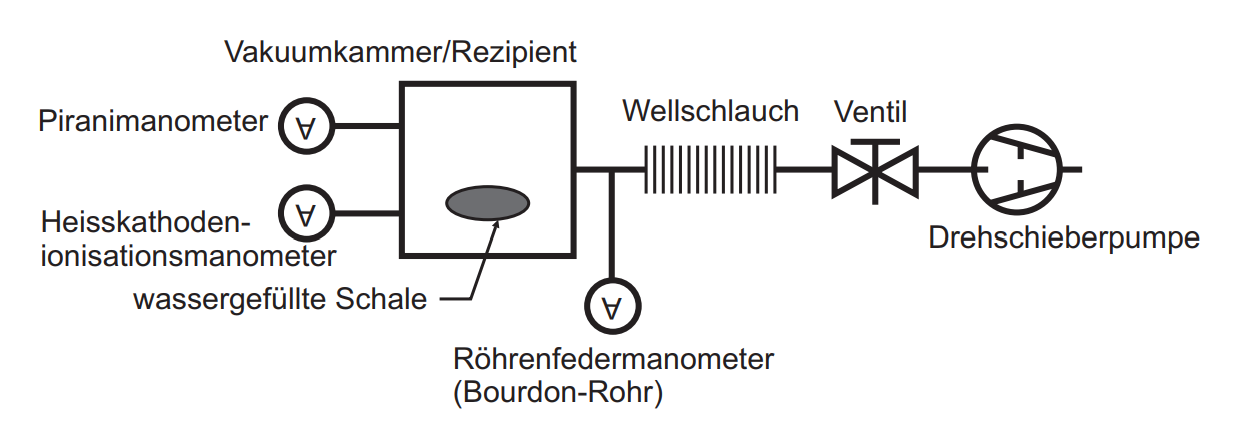
\includegraphics[width=.5\paperwidth]{aufbau22}
            \caption{generalisierter Aufbau zur Beobachtung der Funktionsweise einer Drehschieberpumpe}
            \label{fig:anord1}
        \end{figure}
    
		\begin{figure}[H]
			\centering
			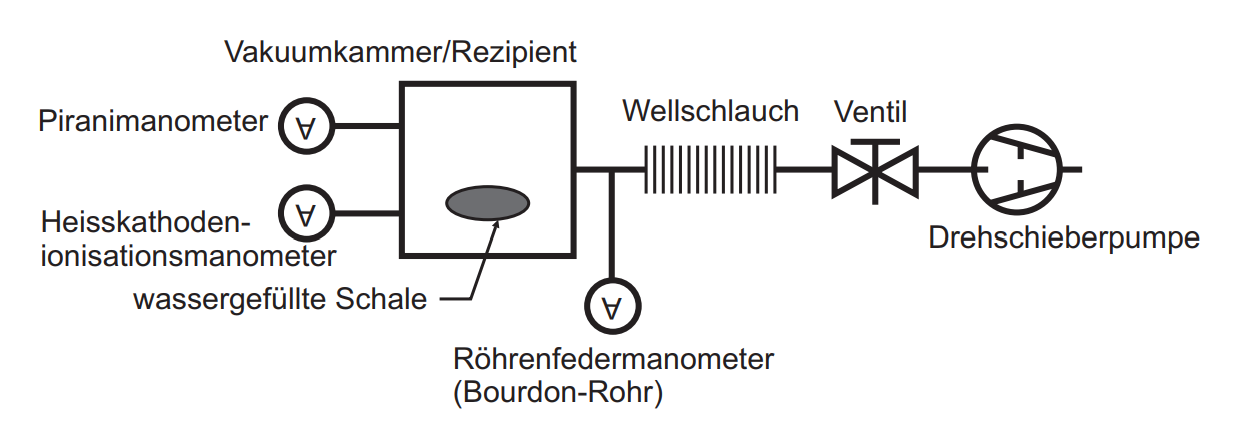
\includegraphics[width=.5\paperwidth]{aufbau22}
			\caption{Vakuum-Blockschaltbild zum Versuch des Abpumpens kondensierbarer Dämpfe}
            \label{fig:anord2}
		\end{figure}
	
        \begin{figure}[H]
            \centering
            %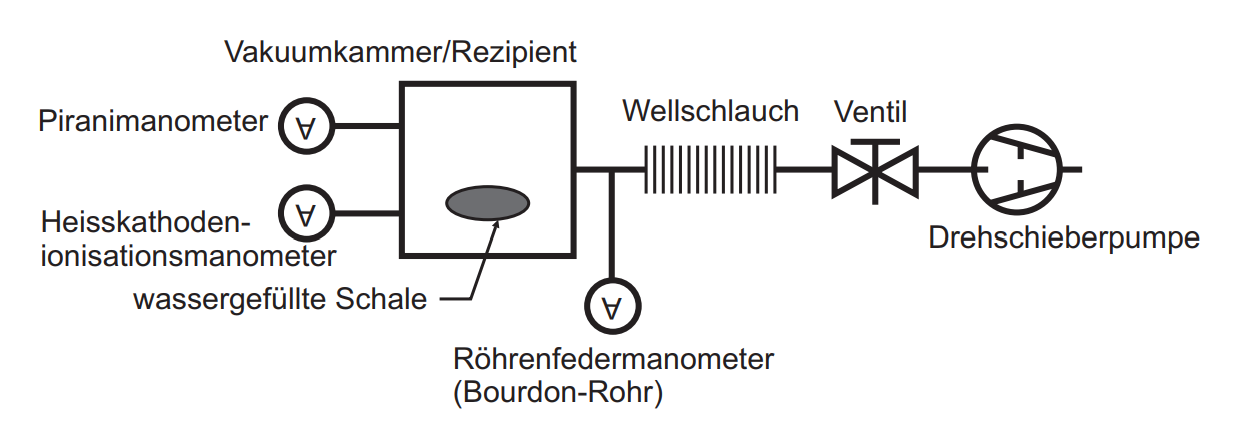
\includegraphics[width=.5\paperwidth]{aufbau22}
            \caption{Aufbau zur Beobachtung der Funktionsweise von Molekular- und Turbomolekularpumpe}
            \label{fig:anord3}
        \end{figure}
    
        \begin{figure}[H]
            \centering
            %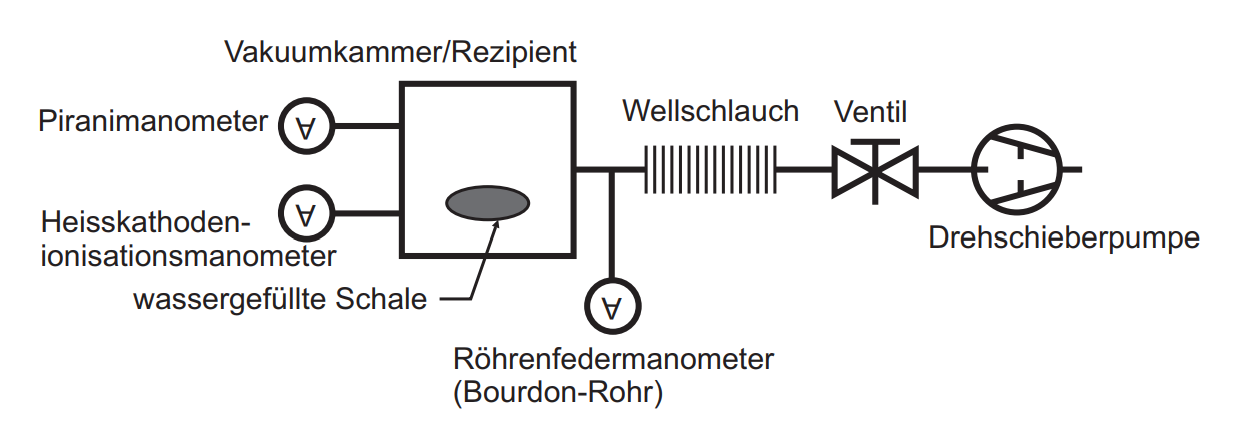
\includegraphics[width=.5\paperwidth]{aufbau22}
            \caption{Bestimmung des Saugvermögens einer TMP}
            \label{fig:anord4}
        \end{figure}
    
        \begin{figure}[H]
            \centering
            %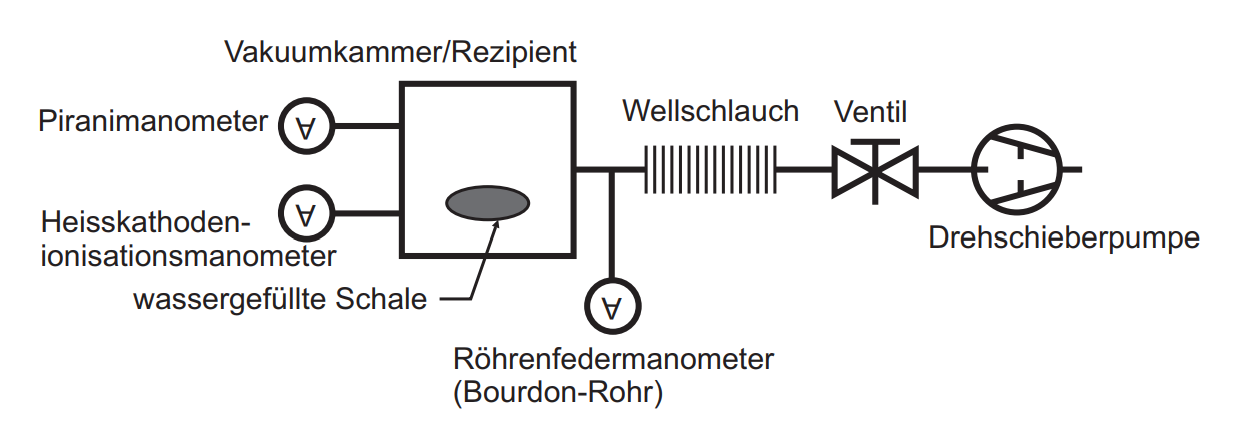
\includegraphics[width=.5\paperwidth]{aufbau22}
            \caption{Aufbau zur Bestimmung des Leitwerts von Rohr und Blende}
            \label{fig:anord5}
        \end{figure}
    
		\begin{figure}[H]
			\centering
			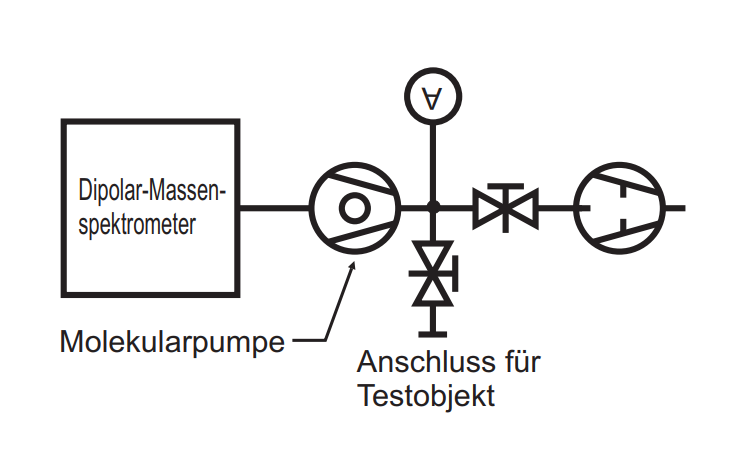
\includegraphics[width=.3\paperwidth]{aufbau262}
			\caption{Prinzipschaltbild des im Versuchsteil 6 eingesetzten Gegenstromlecksuchers}
            \label{fig:anord6}
		\end{figure}
		
	
	\section{Versuchsdurchführung}
	   lnkälknäknöäknknpn
	
	\subsection{Eichung}
	
	
	\section{Ergebnisse}
	
	
	
	\section{Diskussion}
	
	Hier werden alle wesentlichen Ergebnisse nochmals angefuehrt und diskutiert. 
	
	Am Schluss kann man noch eine allgemeinere Bemerkung zum Versuch machen.
	
	
	\newpage 
	
	\begin{thebibliography}{00}   % {00}: max 2-stellig
		
		\bibitem{skript} Versuchsskript zu Versuch F70
		
	\end{thebibliography}
	
\end{document}